
\hypertarget{cv:registrarPantalla}{\section{Registrar Pantalla}} \label{sec:registrarPantalla}

	Esta funcionalidad le permitirá registrar una pantalla dentro del proyecto que se esta operando. 

		\subsection{Procedimiento}

			%Pasos de procedimiento
			\begin{enumerate}
	
			\item Oprima el botón \IURegistrar{} de la pantalla \ref{fig:GestionarPantallas} ''Gestionar Pantallas''.
			
			\item Se mostrará la pantalla \ref{fig:registrarPantalla} ''Registrar Pantalla''.

			%Pantalla
			\begin{figure}[H]
				\begin{center}
					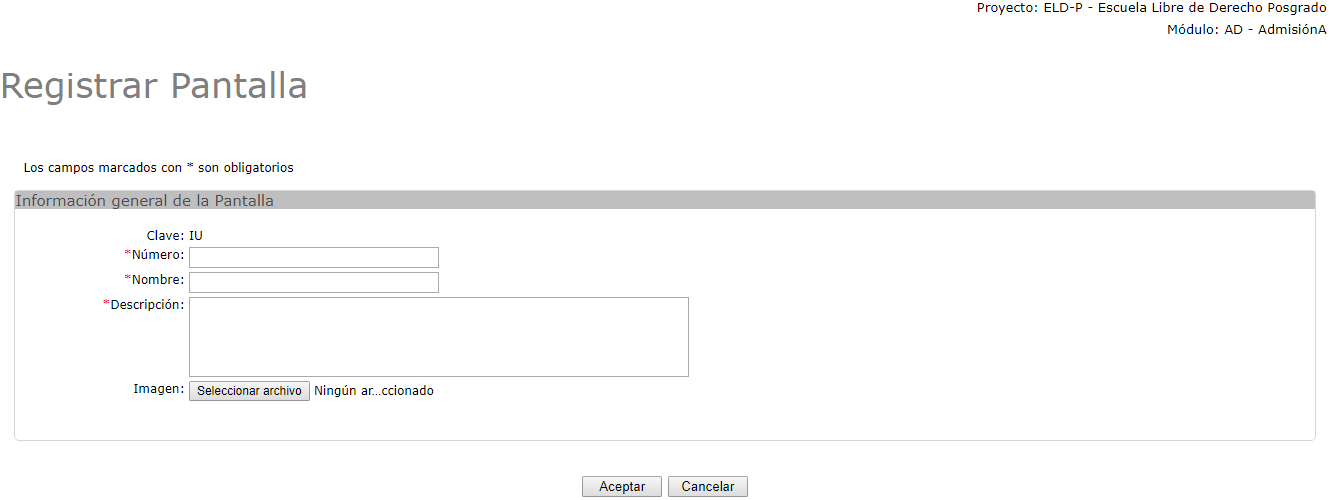
\includegraphics[scale=0.5]{roles/lider/pantallas/pantallas/IU11-1resgitrarPantalla}
					\caption{Registrar Pantalla}
					\label{fig:registrarPantalla}
				\end{center}
			\end{figure}
		
			\item Ingrese el número , el nombre y una pequeña descripción de la pantalla.
			
			\item Adjunte la imagen correspondiente, esta debe pesar como máximo 2 mb y tiene que ser en formato PNG.
			
			\item Oprima el botón \IUAceptar.
			
			\item Se mostrará el mensaje \ref{fig:pantallaRegistrada} en la pantalla \ref{fig:GestionarPantallas} ''Gestionar Pantallas''.
			
			\begin{figure}[htbp!]
				\begin{center}
					
\includegraphics[scale=0.5]{roles/lider/pantallas/pantallas/IU11-1MSG1}
					\caption{MSG: Pantalla Registrada}
					\label{fig:pantallaRegistrada}
				\end{center}
			\end{figure}
			\end{enumerate}